\documentclass[float=false, crop=false]{standalone}
\usepackage[subpreambles=true]{standalone}
\usepackage{import}
\usepackage{geometry}
\geometry{letterpaper, total={146.6mm,246.2mm}, left=25.4mm, top=25.4mm, right=25.4mm, bottom=25.4mm } 		%Total is for writing body space. Left/Right, etc are the margins 
\usepackage{booktabs}
\usepackage{preambleWL}
\usepackage{sidecap}
\newcommand{\titleTemp}{Mushroom Classification}
\lhead{ Winfield Lai 001327375} 			
\chead{ \titleTemp } 					
\rhead{ \today }

\lfoot{ Stats 780 } 		\cfoot{}
\rfoot{Page \thepage}
\linespread{1.25}
\hypersetup{hidelinks}

\begin{document}


\section*{Introduction}

The most interesting question about the Mushroom dataset \cite{UCI} is whether its possible to accurately classify whether a Mushroom is edible or poisonous. This dataset contains hypothetical descriptions of mushrooms. According to the source, there is no simple rule to determine the classification of a mushroom.   Accurately classifying mushrooms has applications dealing with mushroom foragers, and for edible food identification in a desperate survival situation.

The dataset contains 8415 observations, 5935 (3767 Edible, 2168 Poisonous) of which have no missing values. For the purposes of this analysis, observations with missing values were not considered. The response is a classification (Edible or Poisonous) and there are 22 categorical covariates that describe physical characteristics of mushrooms. Several different species (23) of mushrooms are included but no labels exist. Some covariates are slightly subjective (i.e. Odor) but others are not (i.e. CapColor). This is a hypothetical dataset, so all records should be accurate and true. 

\begin{figure}[H] 
		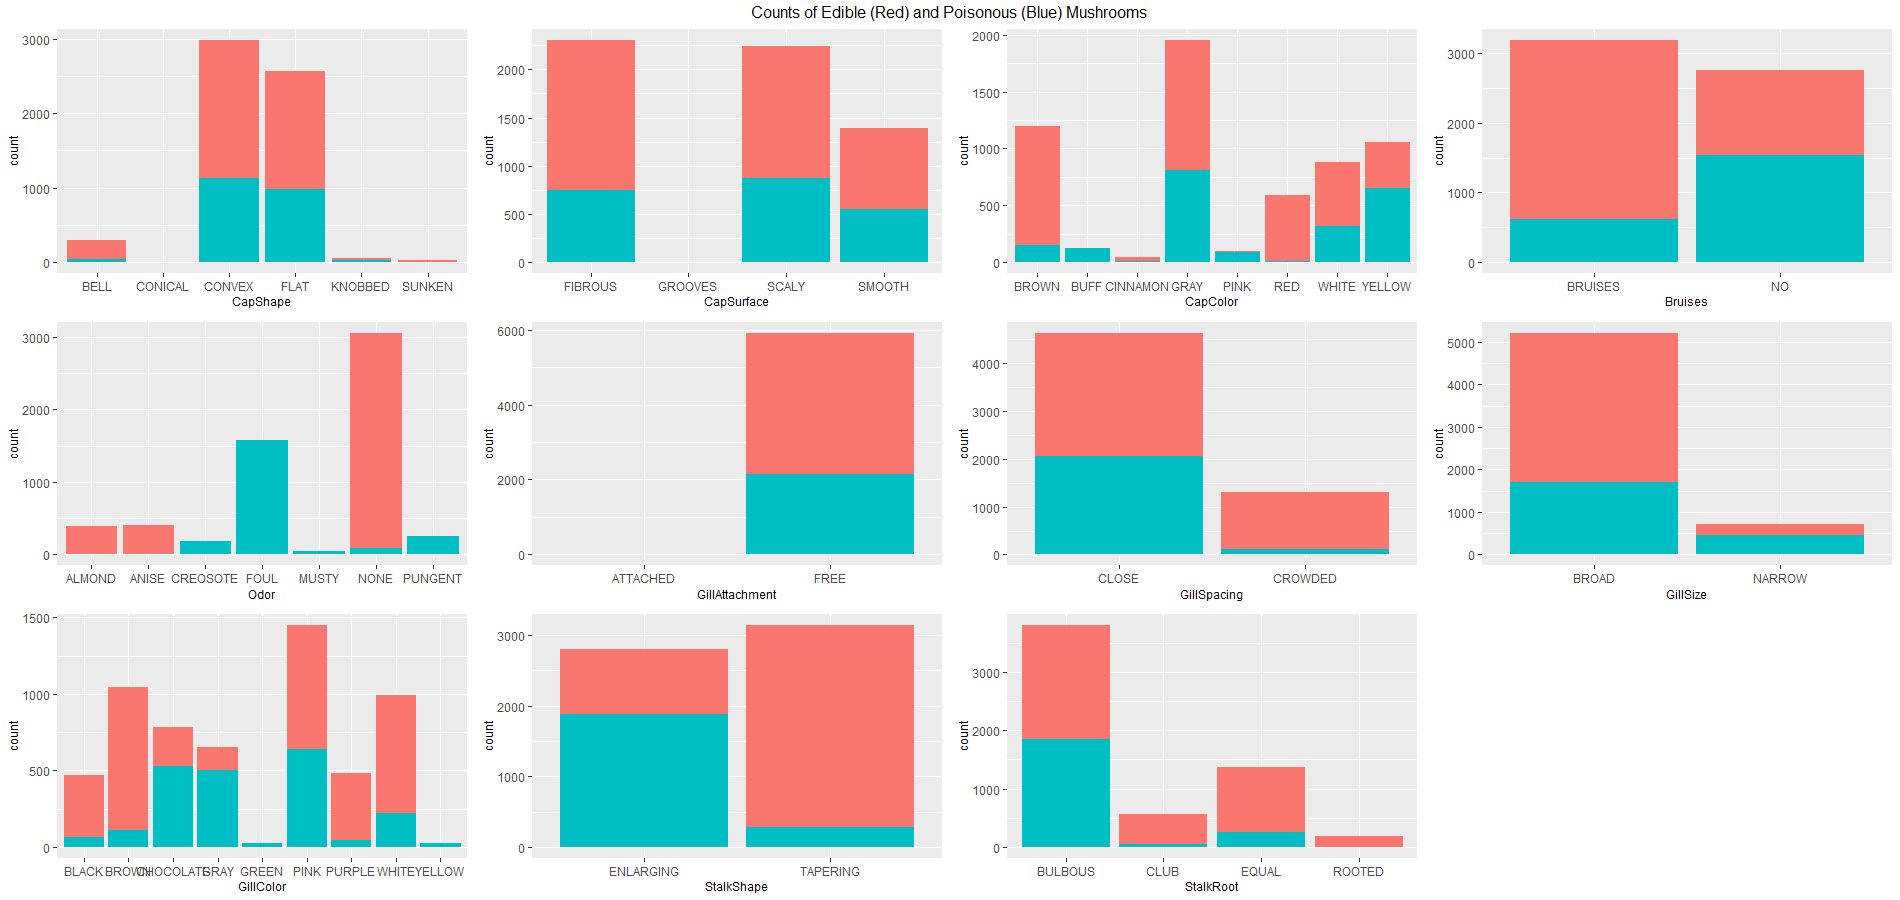
\includegraphics[width=\textwidth, height=5in]{images/stackedbar1.png}
		\caption{Stacked Bar Graph of the Mushroom Dataset. Each graph is a single categorical covariate. Edible Mushrooms are counted in the red bars, Poisonous Mushrooms are counted in the blue bars}
		\label{fig: sbar1}
\end{figure}

\begin{figure}[H] 
		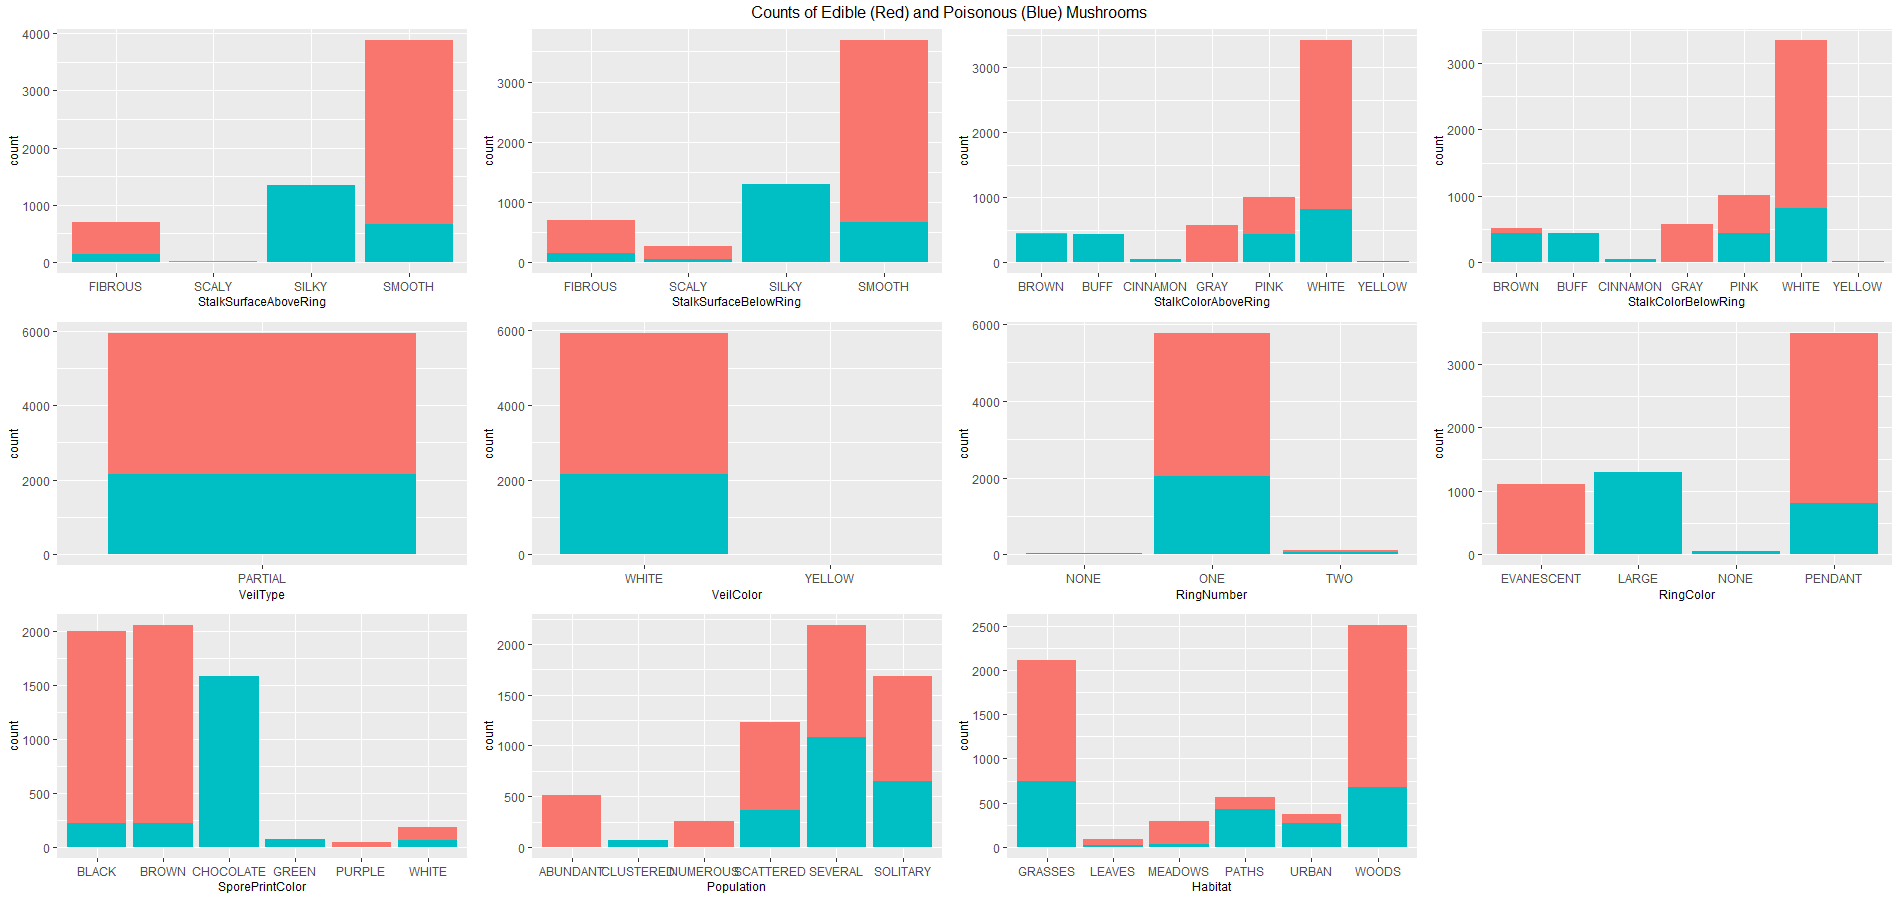
\includegraphics[width=\textwidth, height=5in]{images/stackedbar2.png}
		\caption{Same as Figure 1 but different covariates}
		\label{fig: sbar2}
\end{figure}

Looking at the stacked bar graph above, some covariates (VeilType, VeilColor, maybe RingNumber) provide no meaningful contribution and can be removed. For example, all mushrooms in the dataset have the same VeilType, hence this covariate offers no information that can be used for classification. Some covariates offer good classification - Odor, for example, can be used to almost perfectly classify the data since we see almost complete separation of Edible and Poisonous Mushrooms. 

Most of the covariates have both Edible and Poisonous mushrooms in a single level of the covariate. Hence, these covariates require additional covariates for help in classification. It might be possible that Odor and another covariate perfectly classify this dataset. That would require the second covariate to perfectly classify the overlap of Edible and Poisonous Mushrooms seen in Odor:None bar. 

\section*{Methods}


Variable Reduction was carried out using Association Rules. Association rules were separately calculated for association to only Edible Mushrooms and only Poisonous Mushrooms. The covariates in the top most rule (ordered by standardized lift) were added to the model. The covariates were then removed and Association rules were calculated again to find the next covariates to add to the model. This continued until an average Adjusted Rand Index (ARI) of 1 was obtained by any classification method below. 

Random Forests and Neural Net Classification were used to classify the data. Multiple different ($ > 15 $) $ 50:50 $ training/test sets were used and an average ARI was recorded for each method. R was used for all calculations \cite{Rlang}.

\subsection*{Association Rules}

Association rules are statements where elements of two non-intersecting sets (The covariates and response variables) frequently occur with each other \cite{aRulesLecture}. Association rules are described by notions such as Support, Confidence and Lift. Often, the most useful association rule is above some threshold in Support, Confidence, and Lift. For $ A, B $ being non-intersecting sets of elements from the Covariates and response variables, we have the following. The R package "arules" was used for these calculations \cite{arules1, arules2, arules3} except for standardized lift \cite{standardizedLift}.
%
\begin{flalign} \label{eq: arul1}
\text{Support}		&: s(A \Rightarrow B) = P(A,B) \\
\text{Confidence}	&: c(A \Rightarrow B) = \f{P(A,B)}{P(A)} \\
\text{Lift}			&: L(A \Rightarrow B) = \f{P(A,B)}{P(A)P(B)} 
\end{flalign}
%
Once Association rules have been found and are above the minimum threshold in Support, Confidence and Lift, they are ordered according to some measure of interestingness. In this report, we use the standardized lift to order the association rules. In the equation below, $ s, c $ are the minimum threshold confidence and support. 
%
\begin{flalign} \label{eq: arul2}
\text{Standardized Lift} : 
\mathcal{L} (A \Rightarrow B) 
	&= \f{L(A \Rightarrow B) - \lambda}{v - \lambda} \\
v 
	&= \f{1}{\max\{ P(A), P(B)\}} \\
\lambda 
	&= \max \left\{ 
			\f{P(A) + P(B) - 1}{P(A) P(B)},
			\f{4s}{(1+s)^2},
			\f{s}{P(A)P(B)},
			\f{c}{P(B)}
		\right\} 
\end{flalign}

\subsection*{Adjusted Rand Index}
The Adjusted Rand Index(ARI) is a measure of how well a classification technique has performed \cite{ariLecture}. The ARI takes into account node purity and whether classifications were correct by random chance. If classifications are worse than randomly assignment, the ARI will be negative.
%
\begin{flalign} \label{eq: ari}
%\text{Rand Index (RI)} 			&= \f{A + D}{N} \\
\text{Adjusted Rand Index (ARI)} &= \f{N(A + D) - 
			[(A + B)(A+C) + (C+D)(B+D)]}
		{N^2 - [(A+B)(A+C) + 
			(C+D)(B+D)]}
\end{flalign}
Where $ N = A + B + C + D $ is the total number of pairs between the observations being placed in the correct classification or in the wrong classification. Specifically, $ A $ are the observations correctly classified in the same category, $ B $ are observations wrongly classified as being a different group, $ C $ are observations wrongly classified as the same group and $ D $ are observations correctly classified as the different group. The R package "e1071" was used for these calculations \cite{e1071}.

\subsection*{Random Forest}
Random Forests (RF) uses $ M $ regression or classification trees to make a prediction\cite{forestLecture}. To produce a single prediction, the prediction from the $ M $ classification or regression trees are averaged and hardened in the case of classification trees (Equation below). Each $ M $ tree in a random forest is grown differently. For each tree, bootstrapping is used to re-sample the training set used. Furthermore, only a random subset of the predictor variables are considered for splitting. The R package "randomForest" was used for these calculations \cite{randomForest}.

\begin{flalign} \label{eq: forest}
\hat{f}_{\text{forest}} (x) = \f{1}{M} \s{m=1}{M} \hat{f}_{tree}^m(x)
\end{flalign}


\subsection*{Neural Net}
A neural net is composed of "hidden units" ($ Z_m $) that take into a linear combination of the predictor covariates in order to predict the response \cite{nnetLecture}. Control over the number of hidden units and how they are "activated" for a prediction are key parameters used in a neural net. 
\begin{flalign} \label{eq: nnet}
Z_m 
	&= \sigma(\alpha_{0m} + \alpha_m'\boldsymbol{X}) \\
T_k
	&= \beta_{0k} + \boldsymbol{\beta_k'Z} \\
f_k(\boldsymbol{X})
	&= g_k(\boldsymbol{T}) \\
\boldsymbol{T} &= (T_1, \dots, T_k)' \\
\boldsymbol{Z} &= (Z_1, \dots, Z_m)'
\end{flalign}
where $ M $ is the number of specified hidden units, $ k $ is the number of classes in the response variables, $ \boldsymbol{X} $ is the covariate matrix and $ \alpha_{0m}, \beta_{0k}, \alpha_{m}, \beta_{k} $ are unknown weights that are optimized for. The $ \sigma $ function is an activation function that controls the contribution of each hidden unit to the prediction. $ g_k $ is the output function and transforms the contribution of each hidden unit to get some classification based on the input data. The R package "nnet" was used for these calculations \cite{nnet}


\section*{Results and Discussion}

It is possible to accurately and correctly classify whether a mushroom is poisonous or edible given the covariates/variables. If all variables are included for classification, both unoptimized Random Forest (Split at 6 variables, using 500 trees) and Neural Nets (Size of 5, decay of 0, Max iterations of 100) produce an ARI of 1 for every tested random 50:50 testing/training split. Therefore, we first answer the question of how few variables can be used to achieve a good classification or ARI. 

The average ARI of a number ($ > 15 $) of $ 50:50 $ training/test splits were used to compare different methods and for parameter optimization. Below in Figure \ref{fig: boxAriRed}, we see the boxplots of ARI for Random Forests (same parameters as above) and Neural Nets (same parameters as above). Variables were chosen as described in the methods section. The covariates most associated to the response were added and the new spread of ARI was calculated. Association rules were calculated using a minimum support of 0.055, minimum confidence of 0.8, min length of 2 and max length of 4.
 

\begin{figure}[H]
		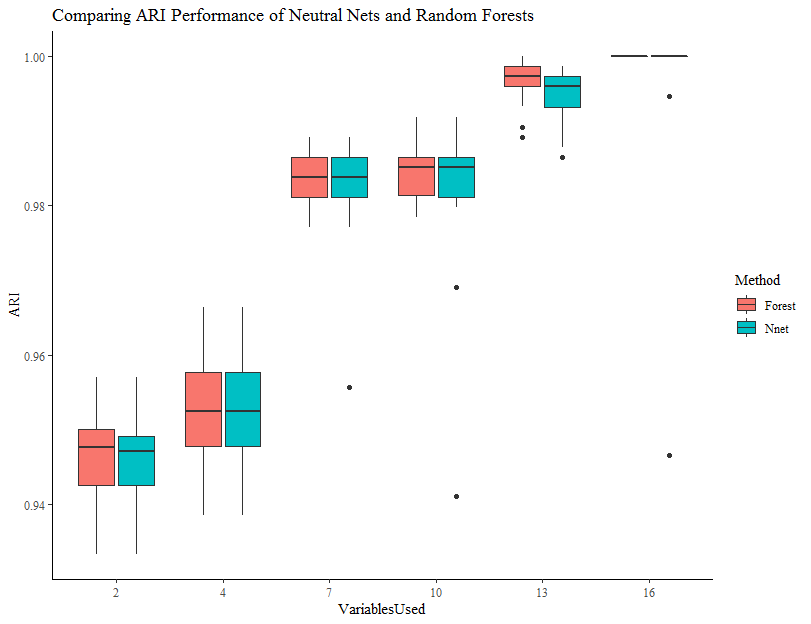
\includegraphics[width=\textwidth, height=4in]{images/boxari.png}
		\caption{Boxplots of the ARI from the Random Forest and Neural Net methods for a changing number of variables used. Each box-plot is composed of 30 ARI points, each using a different 50:50 training/test set.}
		 \label{fig: boxAriRed}
\end{figure}

The figure above indicates that using 2 variables leads to a high ARI and using 16 variables results in a median ARI of 1. Since perfect classification is also possible with 13 variables (Random Forests has a single data point with an ARI of 1), this was the number of variables chosen. Overall, this a reduction from 22 to 13 variables while maintaining an almost perfect classification. If only a high classification was desired, as few as 2 to 7 variables may be used depending on preferences. To see which variables are used, see Figure \ref{fig: parcordRed}. The variables on the bottom are ordered by chronological usage in the Figure 

It's possible that a higher ARI than the one seen in Figure \ref{fig: boxAriRed} can be produced using the same amount of variables. Variables were added by looking at the covariates in association rule with the highest standardized lift. This does not necessarily lead to the fewest number of variables to get a high ARI. This because while the covariates may be highly associated to poisonous or edible mushrooms, they may be associated to the same set of mushrooms. For example, if the top 4 covariates are all associated to the same subset of mushrooms, then using even 1 covariate might lead to the same result. This may be the cause of trend in ARI increase given VariablesUsed. From 2 to 4 and from 7 to 10 variables used, we do not need a significant increase in ARI - the box plot inter quartile ranges are overlapping. 

\begin{figure}[H] 
		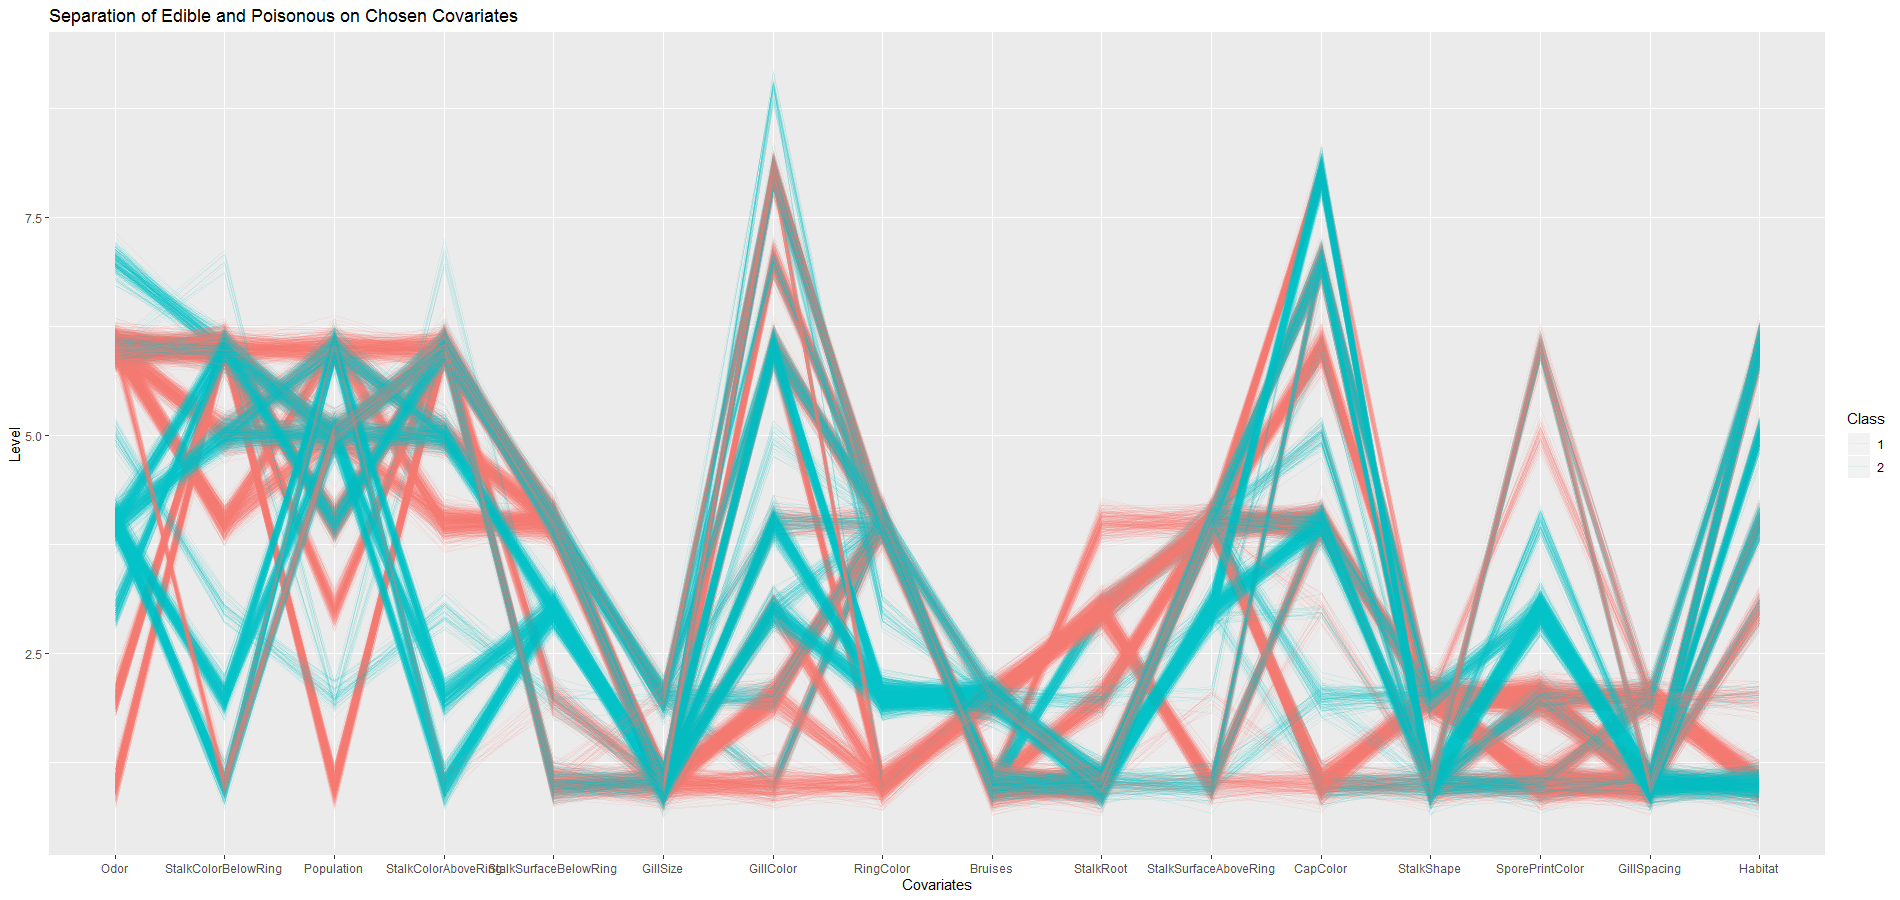
\includegraphics[width=1\textwidth, height=5in]{images/parcord.png}
		\caption{The 16 Variables considered in the the box plot figure above. These variables are in the order of usage by the box plot. In order to see every observation, categorical variables were converted to integers and subsequently had random noise added. This makes every observation unique and also clusters them around the integer representation of the covariate.}
		\label{fig: parcordRed}
\end{figure}

From Figure \ref{fig: parcordRed}, we see that the first 2 variables (same first two variables used in Figure \ref{fig: boxAriRed}) separates out most of the data already. All of the covariates seen in Figure \ref{fig: parcordRed} have at least one level where only one classification of mushroom is present. It's likely the ARI of 1 is obtained when we have a combination of covariates where every observation is in a covariate level that only contains edible or poisonous mushrooms. We see evidence of this in Figure \ref{fig: parcordRed} if we look at some blue lines on the left-most covariate (Odor) as they go to the next covariate (StalkColorBelowRing). 


% latex table generated in R 3.6.1 by xtable 1.8-4 package
% Tue Nov 26 18:34:47 2019
\begin{SCtable} \label{tab: paramNnet}
%\centering
\begin{tabular}{rrrr}
  \hline
  Neural Net&&& \\ 
 Average ARI & Size & Maxit & Decay \\ 
  \hline
0.9970 & 7 & 500 & 0.00 \\ 
  0.9970 & 6 & 300 & 0.25 \\ 
  0.9969 & 2 & 300 & 0.50 \\ 
  0.9968 & 5 & 300 & 0.50 \\ 
  0.9968 & 6 & 300 & 0.00 \\ 
  $\vdots $ & $\vdots $ & $\vdots $ & $\vdots $ \\ 
 0.9773 & 7 & 400 & 0.50 \\ 
  0.9769 & 2 & 200 & 0.25 \\ 
  0.9740 & 4 & 500 & 0.25 \\ 
  0.9738 & 7 & 500 & 0.50 \\ 
  0.9709 & 3 & 400 & 0.25 \\ 
   \hline
\end{tabular}
\caption{Table for parameter optimizations of Neural Net. The table is ordered by decreasing order of Average ARI and only the first and last 5 rows are shown. Average ARI was calculated from 25 50:50 training/test splits. Size was varied from 2 to 7, Maxit was varied from 100 to 500 by jumps of 100 and Decay was varied from 0 to 0.5 by jumps of 0.25. The optimal parameters were at the boundary of the interval used for searching - a larger search interval should have been chosen }
\end{SCtable}

The Neural Net was optimized according to the above table (Optimal parameters are Size = 7, Maxit = 500, Decay = 0). For the parameters checked, the ARI ranged from 0.97 to 0.997. At the optimal value, this is near perfect classification and depending on the training/testing set it could become perfect classification. This is because, as we will see later, the optimal parameters has a single digit number of misclassification out of several thousand predicted classifications. 

\begin{SCtable}\label{tab: paramRf}
%\centering
\begin{tabular}{rrr}
  \hline
  Random Forest&& \\ 
  Average ARI & mTry & nTree \\ 
  \hline
0.9977 & 4 & 350 \\ 
  0.9976 & 3 & 350 \\ 
  0.9976 & 6 & 550 \\ 
  0.9974 & 3 & 500 \\ 
  0.9973 & 9 & 450 \\ 
    $\vdots $ & $\vdots $ & $\vdots $  \\ 
  0.9615 & 1 & 550 \\ 
  0.9612 & 1 & 450 \\ 
  0.9609 & 1 & 600 \\ 
  0.9575 & 1 & 300 \\ 
  0.9571 & 1 & 350 \\ 
   \hline
\end{tabular}
\caption{Random Forest parameter optimization table. The table is ordered by decreasing order of Average ARI and only the first and last 5 rows are shown. Average ARI was calculated from 25 50:50 training/test splits. mTry was varied from 1 to 13, nTree was varied from 300 to 600 by jumps of 50. Note that Bagging was included since we have a maximum of 13 variables to choose from.}
\end{SCtable}


Optimal parameters (mTry = 4, nTree = 350) for Random Forests were found according to the table above. Similar to the Neural Net, Random Forest has near perfect classification. 

\begin{figure}[H] 
		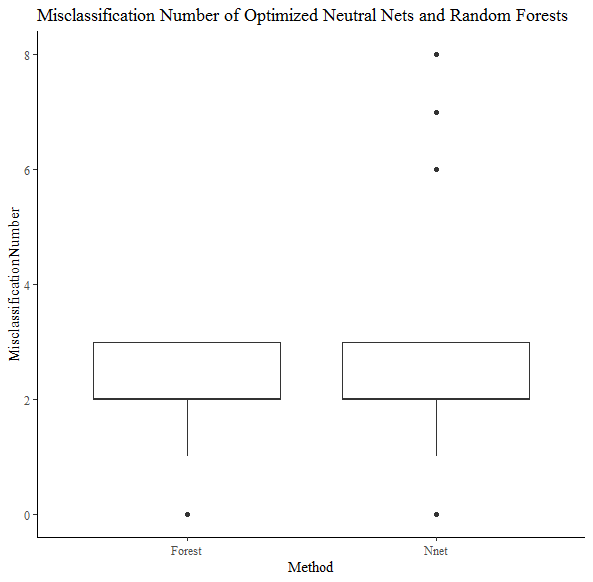
\includegraphics[width=0.5\textwidth, height=3.5in]{images/boxmis.png}
		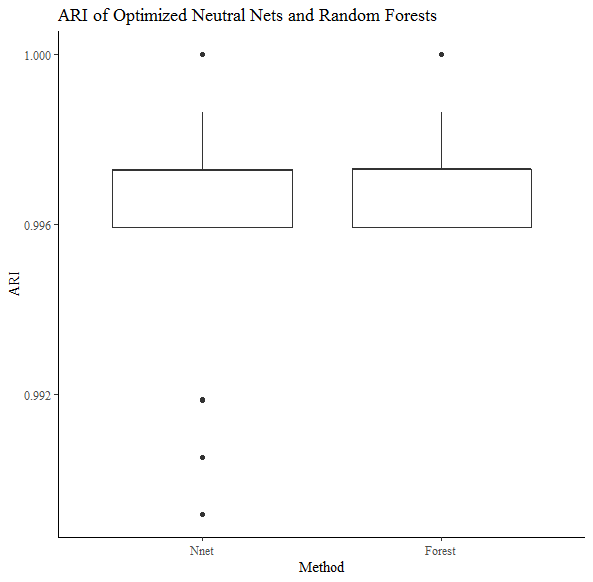
\includegraphics[width=0.5\textwidth, height=3in]{images/boxopt.png}
		\caption{The optimized Neural Net and Random Forest (See above table for parameters) were used on the same 25 50:50 training/test sets (different sets than the one used in method optimization). The box plot of the ARI and total number of misclassifications were plotted.}
		\label{fig: optimout}
\end{figure}

In Figure \ref{fig: optimout}, we have the boxplots of ARI and number of misclassifications for each optimized method. We see that both methods are able to achieve an ARI of 1. More importantly, they have the same median ARI and number of misclassifications but different variances. 

The Neural Net has a higher variance than Random Forests
($ 7.102\cdot 10^{-6} $ vs $ 1.601\cdot 10^{-6} $) albeit both are extremely low. The cause of the huge variance is likely because of how Random Forests calculates predictions. It splits on covariates and from Figure \ref{fig: parcordRed} we know that most of the covariates we have are useful for classifying the data. Thus, most of the trees in the random forest could have different covariates to split on, but will have the same outcome since most covariates are good at splitting the data. This is consistent with Figure \ref{fig: forestvar} since most variables contribute the same amount to the Random Forest (except Odor and the last 2 covariates).

\begin{figure}[H] 
		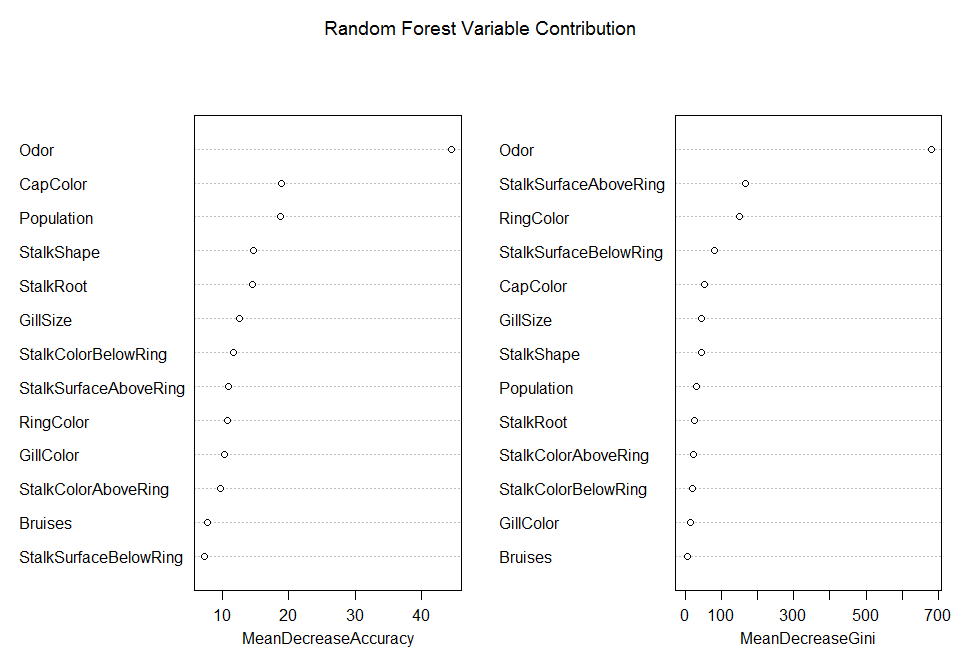
\includegraphics[width=\textwidth, height=4.5in]{images/forestvar.png}
		\caption{The variance contribution of each covariate to the Random Forest. Odor has the biggest contribution to the optimized Random Forest predictions. The next 9 covariates have about equal importance. The 13 variables here were chosen using Association rules described earlier}
		\label{fig: forestvar}
\end{figure}

Nonetheless, both Neural Nets and Random Forests performed extremely well in classifying this dataset. This is due to the fact that every covariate is categorical and many have good separation for the two classifications. Something interesting to do in the future would be to check every single combination of variables and see how few variables are needed until an observation has at least one covariate with a level thats classified as purely edible or purely poisonous. 

Since this is a hypothetical dataset, the relationship between variables here are ideal and the records are not subject to error. If this model is used on real data, we may find that noise introduced from human error in recording observations or from mushrooms not covered in the original dataset will show the model is not as good as near perfect. 

\section*{Conclusion}

A subset of the 22 covariates in the Mushroom Data set is sufficient to achieve perfect classification. Using just 13 covariates (see the covariates listed in Figure \ref{fig: forestvar}), it's possible to achieve an ARI 1. This is guaranteed if we use 16 covariates (see all listed covariates in Figure \ref{fig: parcordRed}). While there is no simple single rule/covariate to classify all the mushrooms, there is one if you look at many covariates.  Variable selection using Association rules does reduce the number variables used however, this may not lead to a minimal set of variables. The most important covariates in classifying is Odor followed by CapColor and Population. 

Neural Nets and Random Forests both perform extremely well at classifying the dataset. Their classifications are on average the same, but the variance of their performance on a train/test set favors Random Forests. The nature of the underlying dataset (ideal hypothetical) likely results in such good separation with the covariates. In a practical situation, the classification may not be as good due to human error on recording data or encountering a mushroom not previously encountered in training set. 

\newpage
\bibliographystyle{plain}
\bibliography{bibtex}



\end{document}
